\clearpage
\section{灯牌的颜色与亮度}
关掉房间里的灯，仍能看见亮着的灯牌。看一块普通木板，眼睛收到的是木板反射过来的光；换成灯牌，表面还会自己发光。在灯牌上的某一点，朝眼睛送出的光 $L_o$ 就是这两份光之和，$L_o=L_r+L_e$。其中 $L_r$ 表示反射光，$L_e$ 表示表面自身发出的光。点光源的阴影可以遮住照向灯牌的光，灯牌上通电的笔画仍然亮着。渲染时先把这两项在线性空间相加，之后才按相机曝光把亮度换成屏幕颜色。

\begin{figure}[H]\centering
\begin{minipage}[b]{.46\linewidth}\centering
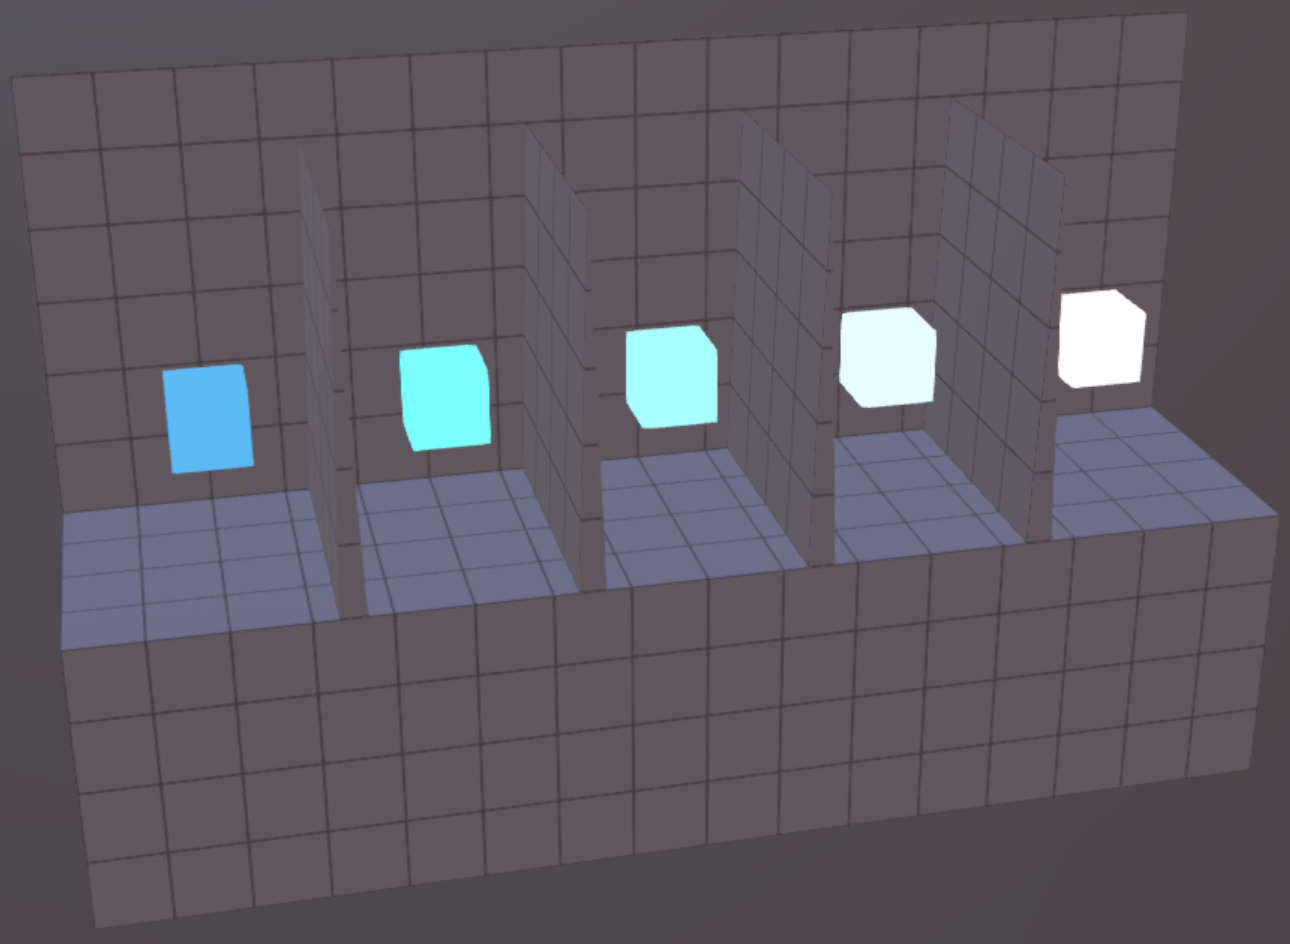
\includegraphics[height=46mm]{figures/emissive-strength-reference.jpg}\\[-1pt]
{\small\sffamily glTF 强度示例}
\end{minipage}\hfill
\begin{minipage}[b]{.51\linewidth}\centering

\includegraphics[height=46mm]{../../../output/profiling/emissive-studio/wide.png}\\[-1pt]
{\small\sffamily Redflag 灯光实验室}
\end{minipage}
\caption{左图五个立方体使用相同的颜色，从左往右将发光强度设为 1、2、4、8、16。原图由 Ed Mackey（AGI，2022）用 BabylonJS 绘制，\href{https://creativecommons.org/licenses/by/4.0/}{CC BY 4.0}。右图来自项目 Vulkan 编辑器的 RenderDoc 回放，三条橙色色带属于同一件材质，中间一条在发光贴图上更暗。}
\end{figure}

右图的材质在 glTF 文件中写着发光因子 $(1,\,0.12,\,0.035)$ 和强度 4。模型导入时把两者相乘，得到材质的 \code{Emission}，即 $(4,\,0.48,\,0.14)$。贴图再控制灯牌的哪些地方亮。白色像素的三个通道都写作 255，乘数是 1；黑色像素的乘数为 0。灰色的 128 在 sRGB 中表示的线性亮度约为 $((128/255+0.055)/1.055)^{2.4}=0.21586$。因此灰带红通道应当是 $4\times0.21586\approx0.86344$，同一配色的 Vulkan 像素测试读到 0.86328。它是曝光前的相对亮度，可以超过 1。

\codewhere{片元着色器节选}{RedflagForge/assets/shaders/Renderer3D_Mesh.glsl}{main}
\begin{lstlisting}
if (u_UseEmissiveMap != 0)
    emission *= texture(u_EmissiveMap, v_EmissiveUV).rgb;
// (*@把这一点自己发出的光加在反射光上。@*)
vec3 color = ambient + Lo + emission;
\end{lstlisting}

没有发光图，整块表面就按材质的发光颜色来画。没有填写发光因子，glTF 默认给黑色。材质的底色和自发光可以分别设定，发光图的透明通道也不会把模型上的笔画挖掉。
\readings{\href{https://github.com/KhronosGroup/glTF-Sample-Assets/tree/main/Models/EmissiveStrengthTest}{Khronos 示例库 · 左图与模型}\quad
\href{https://registry.khronos.org/glTF/specs/2.0/glTF-2.0.html\#additional-textures}{glTF 2.0 §3.9.3}\quad
\href{https://github.com/KhronosGroup/glTF/tree/main/extensions/2.0/Khronos/KHR_materials_emissive_strength}{自发光强度扩展}}

\clearpage
\section{灯牌照到的墙面}
OpenGL 在画灯牌时就知道表面反射了多少光，上一页的加法直接写进场景颜色即可。画许多块灯牌时，同一张贴图可以只选一次，各实例仍各自带一份发光颜色。项目测试摆了四块灯牌，前两块共用网格和贴图，后两块分别没有贴图和使用绿色贴图。实际用了三次主绘制。没有贴图的那块在红通道读到 4，绿色的那块在绿通道读到 2.5，鼠标拾取仍能分辨四块牌子。

Vulkan 编辑器先为每个可见像素记下表面位置、法线和材质，随后才算各处分到了多少光。这 48 字节的数据已经有了各自的用途。遇到实心发光材质时，编辑器另画一张发光图，再把它加进计算好的场景颜色。记录灯牌这次绘制时，原来传底色的三个数可以改传发光颜色，每次绘制的压入常量仍为 128 字节。挡在灯牌前面的物体也参与深度判定，墙后面的灯牌不会盖到墙面上。玻璃则随透明表面按覆盖率合成。

\codewhere{调用节选}{Redflag/src/Platform/Vulkan/Shaders/Emission.frag}{main}
\begin{lstlisting}
// (*@颜色随这次绘制传入；贴图取当前位置的发光图案。@*)
emission.rgb = u_Object.Color.rgb * texture(emissiveMap, v_EmissiveUV).rgb;
\end{lstlisting}

\begin{figure}[H]\centering
\begin{minipage}[b]{.455\linewidth}\centering

\includegraphics[width=\linewidth]{../../../output/profiling/emissive-studio/wall.png}\\[-1pt]
{\small\sffamily 灯牌开启，墙面红通道 0.09709}
\end{minipage}\hspace{4mm}
\begin{minipage}[b]{.455\linewidth}\centering

\includegraphics[width=\linewidth]{../../../output/profiling/emissive-studio/wall-off.png}\\[-1pt]
{\small\sffamily 灯牌关闭，墙面红通道 0}
\end{minipage}
\caption{灯光实验室的两次正式 Vulkan 截帧。从同一位置看白墙，灯牌的四个角都已移出画面。这个场景没有点光源，关掉灯牌以后，白墙就暗了下来。数字取自第 24 帧，在图上距左边 282 像素、距顶边 186 像素处周围 $5\times5$ 个像素取平均。\href{run:../profiling/emissive-studio/frames.json}{原帧与设置}。}
\end{figure}

这时屏幕上的发光图已经看不到灯牌。要把墙照亮，计算间接光的光线仍要能命中镜头外的灯牌。命中一个三角形后，\code{raySurface} 用其三个顶点的贴图坐标插出击中位置的坐标，从发光图取出这一点的颜色。\code{incomingAt} 将它与这块表面反射的光相加。DDGI 把从各方向收到的光存到探针，之后墙面就能查到旁边灯牌送来的光。另用 $17\times17$ 像素测试一面墙，直接对矩形灯牌做面积积分，墙面线性红通道的均值为 0.21522，ReSTIR GI 累积 512 帧后得到 0.21396。

\readings{\src{Redflag/src/Redflag/Renderer/GI/Shaders/GI.comp}{GI.comp · raySurface 与 incomingAt}\quad
\href{run:../profiling/emissive-material/README.md}{显卡读数与像素位置}\\
\href{https://pbr-book.org/4ed/Light_Sources/Area_Lights}{PBRT 第四版 §12.4 · 面光源}\quad
\href{run:../profiling/emissive-gi/measurements.csv}{墙面参考积分与 GPU 实测}}
